%*******************************************************************************
%*********************************** Chapter XXXXXXXX *****************************
%*******************************************************************************

\chapter{Theory}  %Title of chapter

\graphicspath{{Theory/Figs/Raster/}{Theory/Figs/PDF/}{Theory/Figs/Vector/}}

%%% Neutrino physics
\nomenclature[z-CP]{CP}{Charge-Parity}
\nomenclature[z-GUT]{GUT}{Grand Unified Theory}

%%% How LArTPCs gain
\nomenclature[z-Lar]{LAr}{Liquid Argon}
\nomenclature[z-TPC]{TPC}{Time Projection Chamber}
\nomenclature[z-LArTPC]{LArTPC}{Liquid Argon Time Projection Chamber}

%********************************** %First Section  **************************************
\section{Theory of neutrino physics} ~\label{sec:NeutPhys}  %Section - X.1 

%%%% DUNE CDR Volume 2 has a good overview of CP stuff....

%********************************** % Second Section  *************************************
\section{Nucleon decay in Grand Unifying Theories}  \label{sec:Theory_GUT} %Section - X.2

%********************************** % Third Section  *************************************
\section{Background to nucleon decay} \label{sec:BkNDK}  %Section - X.2.3

\begin{figure}
  \centering
  %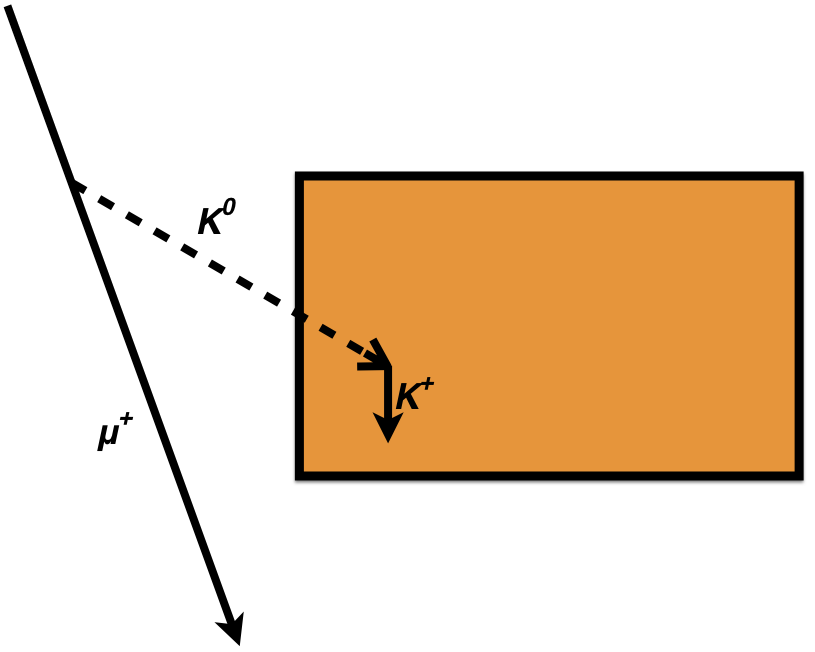
\includegraphics[width=0.5\textwidth]{KaonNDKInteraction}
  \caption[How the interaction of a cosmic muon can mimic a nucleon decay signature]
          {How the interaction of a cosmic muon can mimic a nucleon decay signature, by producing a $K^{0}_{L}$ which interacts far from the detector wall, producing an isolated kaon.}
  \label{fig:K0LongBackground}
\end{figure}


%********************************** %Fourth Section  *************************************
\section{Exisiting and future experiments} \label{sec:Theory_Exp} %Section - X.3

%********************************** %Fifth Section  *************************************
\section{How Liquid Argone Time Projection Chambers work} %Section - X.4
